\documentclass[twoside]{book}

% Packages required by doxygen
\usepackage{calc}
\usepackage{doxygen}
\usepackage{graphicx}
\usepackage[utf8]{inputenc}
\usepackage{makeidx}
\usepackage{multicol}
\usepackage{multirow}
\usepackage{textcomp}
\usepackage[table]{xcolor}

% Font selection
\usepackage[T1]{fontenc}
\usepackage{mathptmx}
\usepackage[scaled=.90]{helvet}
\usepackage{courier}
\usepackage{amssymb}
\usepackage{sectsty}
\renewcommand{\familydefault}{\sfdefault}
\allsectionsfont{%
  \fontseries{bc}\selectfont%
  \color{darkgray}%
}
\renewcommand{\DoxyLabelFont}{%
  \fontseries{bc}\selectfont%
  \color{darkgray}%
}

% Page & text layout
\usepackage{geometry}
\geometry{%
  a4paper,%
  top=2.5cm,%
  bottom=2.5cm,%
  left=2.5cm,%
  right=2.5cm%
}
\tolerance=750
\hfuzz=15pt
\hbadness=750
\setlength{\emergencystretch}{15pt}
\setlength{\parindent}{0cm}
\setlength{\parskip}{0.2cm}
\makeatletter
\renewcommand{\paragraph}{%
  \@startsection{paragraph}{4}{0ex}{-1.0ex}{1.0ex}{%
    \normalfont\normalsize\bfseries\SS@parafont%
  }%
}
\renewcommand{\subparagraph}{%
  \@startsection{subparagraph}{5}{0ex}{-1.0ex}{1.0ex}{%
    \normalfont\normalsize\bfseries\SS@subparafont%
  }%
}
\makeatother

% Headers & footers
\usepackage{fancyhdr}
\pagestyle{fancyplain}
\fancyhead[LE]{\fancyplain{}{\bfseries\thepage}}
\fancyhead[CE]{\fancyplain{}{}}
\fancyhead[RE]{\fancyplain{}{\bfseries\leftmark}}
\fancyhead[LO]{\fancyplain{}{\bfseries\rightmark}}
\fancyhead[CO]{\fancyplain{}{}}
\fancyhead[RO]{\fancyplain{}{\bfseries\thepage}}
\fancyfoot[LE]{\fancyplain{}{}}
\fancyfoot[CE]{\fancyplain{}{}}
\fancyfoot[RE]{\fancyplain{}{\bfseries\scriptsize Generated on Tue Jul 9 2019 22\-:23\-:58 for Effekseer Unity Plugin by Doxygen }}
\fancyfoot[LO]{\fancyplain{}{\bfseries\scriptsize Generated on Tue Jul 9 2019 22\-:23\-:58 for Effekseer Unity Plugin by Doxygen }}
\fancyfoot[CO]{\fancyplain{}{}}
\fancyfoot[RO]{\fancyplain{}{}}
\renewcommand{\footrulewidth}{0.4pt}
\renewcommand{\chaptermark}[1]{%
  \markboth{#1}{}%
}
\renewcommand{\sectionmark}[1]{%
  \markright{\thesection\ #1}%
}

% Indices & bibliography
\usepackage{natbib}
\usepackage[titles]{tocloft}
\setcounter{tocdepth}{3}
\setcounter{secnumdepth}{5}
\makeindex

% Hyperlinks (required, but should be loaded last)
\usepackage{ifpdf}
\ifpdf
  \usepackage[pdftex,pagebackref=true]{hyperref}
\else
  \usepackage[ps2pdf,pagebackref=true]{hyperref}
\fi
\hypersetup{%
  colorlinks=true,%
  linkcolor=blue,%
  citecolor=blue,%
  unicode%
}

% Custom commands
\newcommand{\clearemptydoublepage}{%
  \newpage{\pagestyle{empty}\cleardoublepage}%
}


%===== C O N T E N T S =====

\begin{document}

% Titlepage & ToC
\hypersetup{pageanchor=false}
\pagenumbering{roman}
\begin{titlepage}
\vspace*{7cm}
\begin{center}%
{\Large Effekseer Unity Plugin }\\
\vspace*{1cm}
{\large Generated by Doxygen 1.8.5}\\
\vspace*{0.5cm}
{\small Tue Jul 9 2019 22:23:58}\\
\end{center}
\end{titlepage}
\clearemptydoublepage
\tableofcontents
\clearemptydoublepage
\pagenumbering{arabic}
\hypersetup{pageanchor=true}

%--- Begin generated contents ---
\chapter{Namespace Index}
\section{Namespace List}
Here is a list of all documented namespaces with brief descriptions\-:\begin{DoxyCompactList}
\item\contentsline{section}{\hyperlink{namespace_effekseer}{Effekseer} }{\pageref{namespace_effekseer}}{}
\end{DoxyCompactList}

\chapter{Hierarchical Index}
\doxysection{Class Hierarchy}
This inheritance list is sorted roughly, but not completely, alphabetically\+:\begin{DoxyCompactList}
\item \contentsline{section}{Effekseer.\+Plugin.\+Advanced\+Vertex\+Parameter}{\pageref{struct_effekseer_1_1_plugin_1_1_advanced_vertex_parameter}}{}
\item \contentsline{section}{Effekseer.\+Plugin.\+Edge\+Parameters}{\pageref{struct_effekseer_1_1_plugin_1_1_edge_parameters}}{}
\item \contentsline{section}{Effekseer.\+Effekseer\+System}{\pageref{class_effekseer_1_1_effekseer_system}}{}
\item \contentsline{section}{Effekseer.\+Plugin.\+Falloff\+Parameter}{\pageref{struct_effekseer_1_1_plugin_1_1_falloff_parameter}}{}
\item \contentsline{section}{Effekseer.\+Plugin.\+Flipbook\+Parameters}{\pageref{struct_effekseer_1_1_plugin_1_1_flipbook_parameters}}{}
\item \contentsline{section}{Effekseer.\+Plugin.\+Model\+Face}{\pageref{struct_effekseer_1_1_plugin_1_1_model_face}}{}
\item \contentsline{section}{Effekseer.\+Plugin.\+Model\+Vertex}{\pageref{struct_effekseer_1_1_plugin_1_1_model_vertex}}{}
\item Mono\+Behaviour\begin{DoxyCompactList}
\item \contentsline{section}{Effekseer.\+Effekseer\+Emitter}{\pageref{class_effekseer_1_1_effekseer_emitter}}{}
\end{DoxyCompactList}
\item \contentsline{section}{Effekseer.\+Plugin.\+Stride\+Buffer\+Parameter}{\pageref{struct_effekseer_1_1_plugin_1_1_stride_buffer_parameter}}{}
\item \contentsline{section}{Effekseer.\+Plugin.\+Unity\+Render\+Model\+Parameter1}{\pageref{struct_effekseer_1_1_plugin_1_1_unity_render_model_parameter1}}{}
\item \contentsline{section}{Effekseer.\+Plugin.\+Unity\+Render\+Model\+Parameter2}{\pageref{struct_effekseer_1_1_plugin_1_1_unity_render_model_parameter2}}{}
\item \contentsline{section}{Effekseer.\+Plugin.\+Unity\+Render\+Parameter}{\pageref{struct_effekseer_1_1_plugin_1_1_unity_render_parameter}}{}
\end{DoxyCompactList}

\chapter{Class Index}
\doxysection{Class List}
Here are the classes, structs, unions and interfaces with brief descriptions\+:\begin{DoxyCompactList}
\item\contentsline{section}{\mbox{\hyperlink{struct_effekseer_1_1_plugin_1_1_advanced_vertex_parameter}{Effekseer.\+Plugin.\+Advanced\+Vertex\+Parameter}} }{\pageref{struct_effekseer_1_1_plugin_1_1_advanced_vertex_parameter}}{}
\item\contentsline{section}{\mbox{\hyperlink{struct_effekseer_1_1_plugin_1_1_edge_parameters}{Effekseer.\+Plugin.\+Edge\+Parameters}} }{\pageref{struct_effekseer_1_1_plugin_1_1_edge_parameters}}{}
\item\contentsline{section}{\mbox{\hyperlink{class_effekseer_1_1_effekseer_emitter}{Effekseer.\+Effekseer\+Emitter}} \\*}{\pageref{class_effekseer_1_1_effekseer_emitter}}{}
\item\contentsline{section}{\mbox{\hyperlink{class_effekseer_1_1_effekseer_system}{Effekseer.\+Effekseer\+System}} }{\pageref{class_effekseer_1_1_effekseer_system}}{}
\item\contentsline{section}{\mbox{\hyperlink{struct_effekseer_1_1_plugin_1_1_falloff_parameter}{Effekseer.\+Plugin.\+Falloff\+Parameter}} }{\pageref{struct_effekseer_1_1_plugin_1_1_falloff_parameter}}{}
\item\contentsline{section}{\mbox{\hyperlink{struct_effekseer_1_1_plugin_1_1_flipbook_parameters}{Effekseer.\+Plugin.\+Flipbook\+Parameters}} }{\pageref{struct_effekseer_1_1_plugin_1_1_flipbook_parameters}}{}
\item\contentsline{section}{\mbox{\hyperlink{struct_effekseer_1_1_plugin_1_1_model_face}{Effekseer.\+Plugin.\+Model\+Face}} }{\pageref{struct_effekseer_1_1_plugin_1_1_model_face}}{}
\item\contentsline{section}{\mbox{\hyperlink{struct_effekseer_1_1_plugin_1_1_model_vertex}{Effekseer.\+Plugin.\+Model\+Vertex}} }{\pageref{struct_effekseer_1_1_plugin_1_1_model_vertex}}{}
\item\contentsline{section}{\mbox{\hyperlink{struct_effekseer_1_1_plugin_1_1_stride_buffer_parameter}{Effekseer.\+Plugin.\+Stride\+Buffer\+Parameter}} }{\pageref{struct_effekseer_1_1_plugin_1_1_stride_buffer_parameter}}{}
\item\contentsline{section}{\mbox{\hyperlink{struct_effekseer_1_1_plugin_1_1_unity_render_model_parameter1}{Effekseer.\+Plugin.\+Unity\+Render\+Model\+Parameter1}} \\*Separated buffer (Stride must be lower than 100byte) }{\pageref{struct_effekseer_1_1_plugin_1_1_unity_render_model_parameter1}}{}
\item\contentsline{section}{\mbox{\hyperlink{struct_effekseer_1_1_plugin_1_1_unity_render_model_parameter2}{Effekseer.\+Plugin.\+Unity\+Render\+Model\+Parameter2}} \\*Separated buffer (Stride must be lower than 100byte) }{\pageref{struct_effekseer_1_1_plugin_1_1_unity_render_model_parameter2}}{}
\item\contentsline{section}{\mbox{\hyperlink{struct_effekseer_1_1_plugin_1_1_unity_render_parameter}{Effekseer.\+Plugin.\+Unity\+Render\+Parameter}} }{\pageref{struct_effekseer_1_1_plugin_1_1_unity_render_parameter}}{}
\end{DoxyCompactList}

\chapter{Namespace Documentation}
\hypertarget{namespace_effekseer}{\section{Package Effekseer}
\label{namespace_effekseer}\index{Effekseer@{Effekseer}}
}
\subsection*{Classes}
\begin{DoxyCompactItemize}
\item 
class {\bfseries Resource}
\item 
class {\bfseries Texture\-Resource}
\item 
class {\bfseries Model\-Resource}
\item 
class {\bfseries Sound\-Resource}
\item 
class {\bfseries Utility}
\item 
class {\bfseries Plugin}
\item 
class \hyperlink{class_effekseer_1_1_sound_instance}{Sound\-Instance}
\end{DoxyCompactItemize}

\chapter{Class Documentation}
\hypertarget{class_effekseer_1_1_effekseer_emitter}{\section{Effekseer.\-Effekseer\-Emitter Class Reference}
\label{class_effekseer_1_1_effekseer_emitter}\index{Effekseer.\-Effekseer\-Emitter@{Effekseer.\-Effekseer\-Emitter}}
}
Inheritance diagram for Effekseer.\-Effekseer\-Emitter\-:\begin{figure}[H]
\begin{center}
\leavevmode
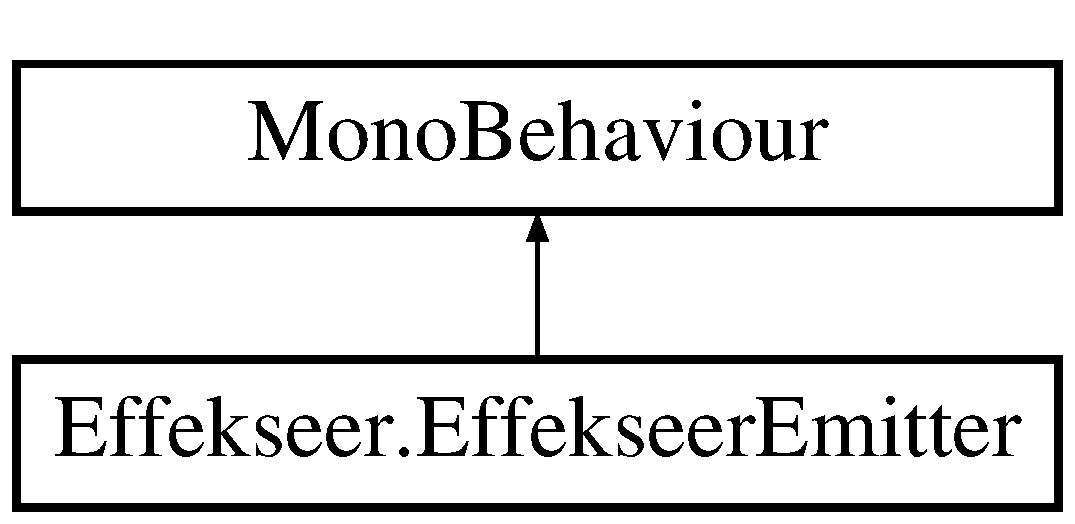
\includegraphics[height=2.000000cm]{class_effekseer_1_1_effekseer_emitter}
\end{center}
\end{figure}
\subsection*{Public Member Functions}
\begin{DoxyCompactItemize}
\item 
Effekseer\-Handle \hyperlink{class_effekseer_1_1_effekseer_emitter_ac06309feaf1798ef0e9553acd75b7ff0}{Play} (Effekseer\-Effect\-Asset \hyperlink{class_effekseer_1_1_effekseer_emitter_abba9195b883a45a4bcc6dcc626173ce9}{effect\-Asset})
\item 
Effekseer\-Handle \hyperlink{class_effekseer_1_1_effekseer_emitter_a82980eeb34709e01cdf5a792e7b4d4c0}{Play} ()
\item 
void \hyperlink{class_effekseer_1_1_effekseer_emitter_a8fe81f1b2f4382e9af35f7cd8722e9d4}{Stop} ()
\item 
void \hyperlink{class_effekseer_1_1_effekseer_emitter_aaf6ca5a2a1a9bc6ed75fd377b415f415}{Stop\-Immediate} ()
\begin{DoxyCompactList}\small\item\em Don't touch it!! \end{DoxyCompactList}\item 
void \hyperlink{class_effekseer_1_1_effekseer_emitter_a49db7f1310c5cab69e72b871c9b666f8}{Stop\-Root} ()
\item 
void \hyperlink{class_effekseer_1_1_effekseer_emitter_a2c3d101b365dfb035f222373958ec3fa}{Set\-All\-Color} (Color color)
\item 
void \hyperlink{class_effekseer_1_1_effekseer_emitter_ac516088d0c7a88124afd5816f103d943}{Set\-Target\-Location} (Vector3 target\-Location)
\item 
void \hyperlink{class_effekseer_1_1_effekseer_emitter_af1bb2b07842a6e671d3c938e4e5ddc28}{Update} ()
\begin{DoxyCompactList}\small\item\em Don't touch it!! \end{DoxyCompactList}\end{DoxyCompactItemize}
\subsection*{Public Attributes}
\begin{DoxyCompactItemize}
\item 
Effekseer\-Effect\-Asset \hyperlink{class_effekseer_1_1_effekseer_emitter_abba9195b883a45a4bcc6dcc626173ce9}{effect\-Asset}
\item 
bool \hyperlink{class_effekseer_1_1_effekseer_emitter_a1ab61ce092db278b2a445078e66a3330}{play\-On\-Start} = false
\item 
bool \hyperlink{class_effekseer_1_1_effekseer_emitter_a99a9a243268bc3fe5e8fa0ea70a85934}{is\-Looping} = false
\item 
List$<$ Effekseer\-Handle $>$ \hyperlink{class_effekseer_1_1_effekseer_emitter_ad7e2bed3f504aa6eb954d0bb95b0353c}{handles} = new List$<$Effekseer\-Handle$>$()
\end{DoxyCompactItemize}
\subsection*{Properties}
\begin{DoxyCompactItemize}
\item 
bool \hyperlink{class_effekseer_1_1_effekseer_emitter_a82833cae53fe0dcb97fe711aae550fd0}{paused}\hspace{0.3cm}{\ttfamily  \mbox{[}get, set\mbox{]}}
\item 
bool \hyperlink{class_effekseer_1_1_effekseer_emitter_af1aadf706ac894eb55fc3cfbf9382294}{shown}\hspace{0.3cm}{\ttfamily  \mbox{[}get, set\mbox{]}}
\item 
float \hyperlink{class_effekseer_1_1_effekseer_emitter_a0cbf08f0a3908780bfbe6933cc5baf1e}{speed}\hspace{0.3cm}{\ttfamily  \mbox{[}get, set\mbox{]}}
\item 
bool \hyperlink{class_effekseer_1_1_effekseer_emitter_ad45907c3a74d2c7d3c6e673788362577}{exists}\hspace{0.3cm}{\ttfamily  \mbox{[}get\mbox{]}}
\end{DoxyCompactItemize}


\subsection{Detailed Description}
$<$summary xml\-:lang=\char`\"{}en\char`\"{}$>$ A emitter of the \hyperlink{namespace_effekseer}{Effekseer} effect 

$<$summary xml\-:lang=\char`\"{}ja\char`\"{}$>$ エフェクトの発生源 

\subsection{Member Function Documentation}
\hypertarget{class_effekseer_1_1_effekseer_emitter_ac06309feaf1798ef0e9553acd75b7ff0}{\index{Effekseer\-::\-Effekseer\-Emitter@{Effekseer\-::\-Effekseer\-Emitter}!Play@{Play}}
\index{Play@{Play}!Effekseer::EffekseerEmitter@{Effekseer\-::\-Effekseer\-Emitter}}
\subsubsection[{Play}]{\setlength{\rightskip}{0pt plus 5cm}Effekseer\-Handle Effekseer.\-Effekseer\-Emitter.\-Play (
\begin{DoxyParamCaption}
\item[{Effekseer\-Effect\-Asset}]{effect\-Asset}
\end{DoxyParamCaption}
)\hspace{0.3cm}{\ttfamily [inline]}}}\label{class_effekseer_1_1_effekseer_emitter_ac06309feaf1798ef0e9553acd75b7ff0}
$<$summary xml\-:lang=\char`\"{}en\char`\"{}$>$ Plays the effect. 
\begin{DoxyParams}{Parameters}
{\em name} & Effect name\\
\hline
\end{DoxyParams}


$<$summary xml\-:lang=\char`\"{}ja\char`\"{}$>$ エフェクトを再生 
\begin{DoxyParams}{Parameters}
{\em name} & エフェクト名\\
\hline
\end{DoxyParams}
\hypertarget{class_effekseer_1_1_effekseer_emitter_a82980eeb34709e01cdf5a792e7b4d4c0}{\index{Effekseer\-::\-Effekseer\-Emitter@{Effekseer\-::\-Effekseer\-Emitter}!Play@{Play}}
\index{Play@{Play}!Effekseer::EffekseerEmitter@{Effekseer\-::\-Effekseer\-Emitter}}
\subsubsection[{Play}]{\setlength{\rightskip}{0pt plus 5cm}Effekseer\-Handle Effekseer.\-Effekseer\-Emitter.\-Play (
\begin{DoxyParamCaption}
{}
\end{DoxyParamCaption}
)\hspace{0.3cm}{\ttfamily [inline]}}}\label{class_effekseer_1_1_effekseer_emitter_a82980eeb34709e01cdf5a792e7b4d4c0}
$<$summary xml\-:lang=\char`\"{}en\char`\"{}$>$ Plays the effect that has been set. 

$<$summary xml\-:lang=\char`\"{}ja\char`\"{}$>$ 設定されているエフェクトを再生 \hypertarget{class_effekseer_1_1_effekseer_emitter_a2c3d101b365dfb035f222373958ec3fa}{\index{Effekseer\-::\-Effekseer\-Emitter@{Effekseer\-::\-Effekseer\-Emitter}!Set\-All\-Color@{Set\-All\-Color}}
\index{Set\-All\-Color@{Set\-All\-Color}!Effekseer::EffekseerEmitter@{Effekseer\-::\-Effekseer\-Emitter}}
\subsubsection[{Set\-All\-Color}]{\setlength{\rightskip}{0pt plus 5cm}void Effekseer.\-Effekseer\-Emitter.\-Set\-All\-Color (
\begin{DoxyParamCaption}
\item[{Color}]{color}
\end{DoxyParamCaption}
)\hspace{0.3cm}{\ttfamily [inline]}}}\label{class_effekseer_1_1_effekseer_emitter_a2c3d101b365dfb035f222373958ec3fa}
$<$summary xml\-:lang=\char`\"{}en\char`\"{}$>$ Specify the color of overall effect. 

$<$summary xml\-:lang=\char`\"{}ja\char`\"{}$>$ エフェクト全体の色を指定する。 


\begin{DoxyParams}{Parameters}
{\em color} & Color\\
\hline
\end{DoxyParams}
\hypertarget{class_effekseer_1_1_effekseer_emitter_ac516088d0c7a88124afd5816f103d943}{\index{Effekseer\-::\-Effekseer\-Emitter@{Effekseer\-::\-Effekseer\-Emitter}!Set\-Target\-Location@{Set\-Target\-Location}}
\index{Set\-Target\-Location@{Set\-Target\-Location}!Effekseer::EffekseerEmitter@{Effekseer\-::\-Effekseer\-Emitter}}
\subsubsection[{Set\-Target\-Location}]{\setlength{\rightskip}{0pt plus 5cm}void Effekseer.\-Effekseer\-Emitter.\-Set\-Target\-Location (
\begin{DoxyParamCaption}
\item[{Vector3}]{target\-Location}
\end{DoxyParamCaption}
)\hspace{0.3cm}{\ttfamily [inline]}}}\label{class_effekseer_1_1_effekseer_emitter_ac516088d0c7a88124afd5816f103d943}
$<$summary xml\-:lang=\char`\"{}en\char`\"{}$>$ Sets the target location of the played effects. $<$param name=\char`\"{}target\-Location\char`\"{} xml\-:lang=\char`\"{}en\char`\"{}$>$Target location

$<$summary xml\-:lang=\char`\"{}ja\char`\"{}$>$ 再生中のエフェクトのターゲット位置を設定 $<$param name=\char`\"{}target\-Location\char`\"{} xml\-:lang=\char`\"{}ja\char`\"{}$>$ターゲット位置\hypertarget{class_effekseer_1_1_effekseer_emitter_a8fe81f1b2f4382e9af35f7cd8722e9d4}{\index{Effekseer\-::\-Effekseer\-Emitter@{Effekseer\-::\-Effekseer\-Emitter}!Stop@{Stop}}
\index{Stop@{Stop}!Effekseer::EffekseerEmitter@{Effekseer\-::\-Effekseer\-Emitter}}
\subsubsection[{Stop}]{\setlength{\rightskip}{0pt plus 5cm}void Effekseer.\-Effekseer\-Emitter.\-Stop (
\begin{DoxyParamCaption}
{}
\end{DoxyParamCaption}
)\hspace{0.3cm}{\ttfamily [inline]}}}\label{class_effekseer_1_1_effekseer_emitter_a8fe81f1b2f4382e9af35f7cd8722e9d4}
$<$summary xml\-:lang=\char`\"{}en\char`\"{}$>$ Stops the played effect. All nodes will be destroyed. 

$<$summary xml\-:lang=\char`\"{}ja\char`\"{}$>$ 再生中のエフェクトを停止 全てのノードが即座に消える \hypertarget{class_effekseer_1_1_effekseer_emitter_aaf6ca5a2a1a9bc6ed75fd377b415f415}{\index{Effekseer\-::\-Effekseer\-Emitter@{Effekseer\-::\-Effekseer\-Emitter}!Stop\-Immediate@{Stop\-Immediate}}
\index{Stop\-Immediate@{Stop\-Immediate}!Effekseer::EffekseerEmitter@{Effekseer\-::\-Effekseer\-Emitter}}
\subsubsection[{Stop\-Immediate}]{\setlength{\rightskip}{0pt plus 5cm}void Effekseer.\-Effekseer\-Emitter.\-Stop\-Immediate (
\begin{DoxyParamCaption}
{}
\end{DoxyParamCaption}
)\hspace{0.3cm}{\ttfamily [inline]}}}\label{class_effekseer_1_1_effekseer_emitter_aaf6ca5a2a1a9bc6ed75fd377b415f415}


Don't touch it!! 

\hypertarget{class_effekseer_1_1_effekseer_emitter_a49db7f1310c5cab69e72b871c9b666f8}{\index{Effekseer\-::\-Effekseer\-Emitter@{Effekseer\-::\-Effekseer\-Emitter}!Stop\-Root@{Stop\-Root}}
\index{Stop\-Root@{Stop\-Root}!Effekseer::EffekseerEmitter@{Effekseer\-::\-Effekseer\-Emitter}}
\subsubsection[{Stop\-Root}]{\setlength{\rightskip}{0pt plus 5cm}void Effekseer.\-Effekseer\-Emitter.\-Stop\-Root (
\begin{DoxyParamCaption}
{}
\end{DoxyParamCaption}
)\hspace{0.3cm}{\ttfamily [inline]}}}\label{class_effekseer_1_1_effekseer_emitter_a49db7f1310c5cab69e72b871c9b666f8}
$<$summary xml\-:lang=\char`\"{}en\char`\"{}$>$ Stops the root node of the played effect. The root node will be destroyed. Then children also will be destroyed by their lifetime. 

$<$summary xml\-:lang=\char`\"{}ja\char`\"{}$>$ 再生中のエフェクトのルートノードだけを停止 ルートノードを削除したことで子ノード生成が停止され寿命で徐々に消える \hypertarget{class_effekseer_1_1_effekseer_emitter_af1bb2b07842a6e671d3c938e4e5ddc28}{\index{Effekseer\-::\-Effekseer\-Emitter@{Effekseer\-::\-Effekseer\-Emitter}!Update@{Update}}
\index{Update@{Update}!Effekseer::EffekseerEmitter@{Effekseer\-::\-Effekseer\-Emitter}}
\subsubsection[{Update}]{\setlength{\rightskip}{0pt plus 5cm}void Effekseer.\-Effekseer\-Emitter.\-Update (
\begin{DoxyParamCaption}
{}
\end{DoxyParamCaption}
)\hspace{0.3cm}{\ttfamily [inline]}}}\label{class_effekseer_1_1_effekseer_emitter_af1bb2b07842a6e671d3c938e4e5ddc28}


Don't touch it!! 



\subsection{Member Data Documentation}
\hypertarget{class_effekseer_1_1_effekseer_emitter_abba9195b883a45a4bcc6dcc626173ce9}{\index{Effekseer\-::\-Effekseer\-Emitter@{Effekseer\-::\-Effekseer\-Emitter}!effect\-Asset@{effect\-Asset}}
\index{effect\-Asset@{effect\-Asset}!Effekseer::EffekseerEmitter@{Effekseer\-::\-Effekseer\-Emitter}}
\subsubsection[{effect\-Asset}]{\setlength{\rightskip}{0pt plus 5cm}Effekseer\-Effect\-Asset Effekseer.\-Effekseer\-Emitter.\-effect\-Asset}}\label{class_effekseer_1_1_effekseer_emitter_abba9195b883a45a4bcc6dcc626173ce9}
$<$summary xml\-:lang=\char`\"{}en\char`\"{}$>$ Effect name 

$<$summary xml\-:lang=\char`\"{}ja\char`\"{}$>$ エフェクト名 

$<$summary xml\-:lang=\char`\"{}en\char`\"{}$>$ Effect name 

$<$summary xml\-:lang=\char`\"{}ja\char`\"{}$>$ エフェクト名 \hypertarget{class_effekseer_1_1_effekseer_emitter_ad7e2bed3f504aa6eb954d0bb95b0353c}{\index{Effekseer\-::\-Effekseer\-Emitter@{Effekseer\-::\-Effekseer\-Emitter}!handles@{handles}}
\index{handles@{handles}!Effekseer::EffekseerEmitter@{Effekseer\-::\-Effekseer\-Emitter}}
\subsubsection[{handles}]{\setlength{\rightskip}{0pt plus 5cm}List$<$Effekseer\-Handle$>$ Effekseer.\-Effekseer\-Emitter.\-handles = new List$<$Effekseer\-Handle$>$()}}\label{class_effekseer_1_1_effekseer_emitter_ad7e2bed3f504aa6eb954d0bb95b0353c}
$<$summary xml\-:lang=\char`\"{}en\char`\"{}$>$ The last played handle. Don't touch it!! 

$<$summary xml\-:lang=\char`\"{}ja\char`\"{}$>$ 最後に\-Playされたハンドル Effekseer開発者以外は触ってはいけない \hypertarget{class_effekseer_1_1_effekseer_emitter_a99a9a243268bc3fe5e8fa0ea70a85934}{\index{Effekseer\-::\-Effekseer\-Emitter@{Effekseer\-::\-Effekseer\-Emitter}!is\-Looping@{is\-Looping}}
\index{is\-Looping@{is\-Looping}!Effekseer::EffekseerEmitter@{Effekseer\-::\-Effekseer\-Emitter}}
\subsubsection[{is\-Looping}]{\setlength{\rightskip}{0pt plus 5cm}bool Effekseer.\-Effekseer\-Emitter.\-is\-Looping = false}}\label{class_effekseer_1_1_effekseer_emitter_a99a9a243268bc3fe5e8fa0ea70a85934}
$<$summary xml\-:lang=\char`\"{}ja\char`\"{}$>$ Whether it does loop playback when all effects are stopped 

$<$summary xml\-:lang=\char`\"{}ja\char`\"{}$>$ 全てのエフェクトが停止した後に、ループ再生するかどうか \hypertarget{class_effekseer_1_1_effekseer_emitter_a1ab61ce092db278b2a445078e66a3330}{\index{Effekseer\-::\-Effekseer\-Emitter@{Effekseer\-::\-Effekseer\-Emitter}!play\-On\-Start@{play\-On\-Start}}
\index{play\-On\-Start@{play\-On\-Start}!Effekseer::EffekseerEmitter@{Effekseer\-::\-Effekseer\-Emitter}}
\subsubsection[{play\-On\-Start}]{\setlength{\rightskip}{0pt plus 5cm}bool Effekseer.\-Effekseer\-Emitter.\-play\-On\-Start = false}}\label{class_effekseer_1_1_effekseer_emitter_a1ab61ce092db278b2a445078e66a3330}
$<$summary xml\-:lang=\char`\"{}en\char`\"{}$>$ Whether it does play the effect on Start() 

$<$summary xml\-:lang=\char`\"{}ja\char`\"{}$>$ Start()時に再生開始するかどうか 

\subsection{Property Documentation}
\hypertarget{class_effekseer_1_1_effekseer_emitter_ad45907c3a74d2c7d3c6e673788362577}{\index{Effekseer\-::\-Effekseer\-Emitter@{Effekseer\-::\-Effekseer\-Emitter}!exists@{exists}}
\index{exists@{exists}!Effekseer::EffekseerEmitter@{Effekseer\-::\-Effekseer\-Emitter}}
\subsubsection[{exists}]{\setlength{\rightskip}{0pt plus 5cm}bool Effekseer.\-Effekseer\-Emitter.\-exists\hspace{0.3cm}{\ttfamily [get]}}}\label{class_effekseer_1_1_effekseer_emitter_ad45907c3a74d2c7d3c6e673788362577}
$<$summary xml\-:lang=\char`\"{}en\char`\"{}$>$ Existing state 

true\-: It's existed.

false\-: It isn't existed or stopped.

$<$summary xml\-:lang=\char`\"{}ja\char`\"{}$>$ 再生中のエフェクトが存在しているか 

true\-: 存在している

false\-: 再生終了で破棄。もしくは\-Stopで停止された\hypertarget{class_effekseer_1_1_effekseer_emitter_a82833cae53fe0dcb97fe711aae550fd0}{\index{Effekseer\-::\-Effekseer\-Emitter@{Effekseer\-::\-Effekseer\-Emitter}!paused@{paused}}
\index{paused@{paused}!Effekseer::EffekseerEmitter@{Effekseer\-::\-Effekseer\-Emitter}}
\subsubsection[{paused}]{\setlength{\rightskip}{0pt plus 5cm}bool Effekseer.\-Effekseer\-Emitter.\-paused\hspace{0.3cm}{\ttfamily [get]}, {\ttfamily [set]}}}\label{class_effekseer_1_1_effekseer_emitter_a82833cae53fe0dcb97fe711aae550fd0}
$<$summary xml\-:lang=\char`\"{}en\char`\"{}$>$ Pausing the effect 

true\-: It will update on \hyperlink{class_effekseer_1_1_effekseer_emitter_af1bb2b07842a6e671d3c938e4e5ddc28}{Update()}

false\-: It will not update on \hyperlink{class_effekseer_1_1_effekseer_emitter_af1bb2b07842a6e671d3c938e4e5ddc28}{Update()}

$<$summary xml\-:lang=\char`\"{}ja\char`\"{}$>$ ポーズ設定 

true\-: Updateで更新しない

false\-: Updateで更新する\hypertarget{class_effekseer_1_1_effekseer_emitter_af1aadf706ac894eb55fc3cfbf9382294}{\index{Effekseer\-::\-Effekseer\-Emitter@{Effekseer\-::\-Effekseer\-Emitter}!shown@{shown}}
\index{shown@{shown}!Effekseer::EffekseerEmitter@{Effekseer\-::\-Effekseer\-Emitter}}
\subsubsection[{shown}]{\setlength{\rightskip}{0pt plus 5cm}bool Effekseer.\-Effekseer\-Emitter.\-shown\hspace{0.3cm}{\ttfamily [get]}, {\ttfamily [set]}}}\label{class_effekseer_1_1_effekseer_emitter_af1aadf706ac894eb55fc3cfbf9382294}
$<$summary xml\-:lang=\char`\"{}en\char`\"{}$>$ Showing the effect 

true\-: It will be rendering.

false\-: It will not be rendering.

$<$summary xml\-:lang=\char`\"{}ja\char`\"{}$>$ 表示設定 

true\-: 描画する

false\-: 描画しない\hypertarget{class_effekseer_1_1_effekseer_emitter_a0cbf08f0a3908780bfbe6933cc5baf1e}{\index{Effekseer\-::\-Effekseer\-Emitter@{Effekseer\-::\-Effekseer\-Emitter}!speed@{speed}}
\index{speed@{speed}!Effekseer::EffekseerEmitter@{Effekseer\-::\-Effekseer\-Emitter}}
\subsubsection[{speed}]{\setlength{\rightskip}{0pt plus 5cm}float Effekseer.\-Effekseer\-Emitter.\-speed\hspace{0.3cm}{\ttfamily [get]}, {\ttfamily [set]}}}\label{class_effekseer_1_1_effekseer_emitter_a0cbf08f0a3908780bfbe6933cc5baf1e}
$<$summary xml\-:lang=\char`\"{}en\char`\"{}$>$ Playback speed 

$<$summary xml\-:lang=\char`\"{}ja\char`\"{}$>$ 再生速度 

The documentation for this class was generated from the following file\-:\begin{DoxyCompactItemize}
\item 
D\-:/dev/\-\_\-\-Effekseer/\-Effekseer14x/\-Effekseer\-For\-Unity/\-Dev/\-Plugin/\-Assets/\-Effekseer/\-Scripts/Effekseer\-Emitter.\-cs\end{DoxyCompactItemize}

\hypertarget{class_effekseer_1_1_effekseer_system}{\section{Effekseer.\-Effekseer\-System Class Reference}
\label{class_effekseer_1_1_effekseer_system}\index{Effekseer.\-Effekseer\-System@{Effekseer.\-Effekseer\-System}}
}
\subsection*{Public Member Functions}
\begin{DoxyCompactItemize}
\item 
void \hyperlink{class_effekseer_1_1_effekseer_system_a9fd8b0498b1652552d562a84890acd8e}{Load\-Effect} (Effekseer\-Effect\-Asset effect\-Asset)
\begin{DoxyCompactList}\small\item\em Don't touch it!! \end{DoxyCompactList}\item 
void \hyperlink{class_effekseer_1_1_effekseer_system_a9f9623f5c80cb4ad197aaa0ea8e185bd}{Init\-Plugin} ()
\begin{DoxyCompactList}\small\item\em Don't touch it!! \end{DoxyCompactList}\item 
void \hyperlink{class_effekseer_1_1_effekseer_system_af1da0db69f6c0a2bb68ce459322078bf}{Term\-Plugin} ()
\begin{DoxyCompactList}\small\item\em Don't touch it!! \end{DoxyCompactList}\item 
void \hyperlink{class_effekseer_1_1_effekseer_system_ae53076ec94edc395e8e422c8f16fdf2e}{On\-Enable} ()
\begin{DoxyCompactList}\small\item\em Don't touch it!! \end{DoxyCompactList}\item 
void \hyperlink{class_effekseer_1_1_effekseer_system_a7a743450e7242c812ccb4d556f3a8a43}{On\-Disable} ()
\begin{DoxyCompactList}\small\item\em Don't touch it!! \end{DoxyCompactList}\end{DoxyCompactItemize}
\subsection*{Static Public Member Functions}
\begin{DoxyCompactItemize}
\item 
static Effekseer\-Handle \hyperlink{class_effekseer_1_1_effekseer_system_a679e2cbf7d99ff2af5db1608e82e9201}{Play\-Effect} (Effekseer\-Effect\-Asset effect\-Asset, Vector3 location)
\item 
static void \hyperlink{class_effekseer_1_1_effekseer_system_a9431e338ba62ded97108c1c04d05ed98}{Stop\-All\-Effects} ()
\item 
static void \hyperlink{class_effekseer_1_1_effekseer_system_adfbdc2b070592e412eb6b560865be455}{Set\-Paused\-To\-All\-Effects} (bool paused)
\item 
static bool \hyperlink{class_effekseer_1_1_effekseer_system_a15a902264fbb68ec2b79bed290175ac9}{Start\-Network} ()
\item 
static void \hyperlink{class_effekseer_1_1_effekseer_system_ae3e8a328c72789ef63670668525b255c}{Stop\-Network} ()
\end{DoxyCompactItemize}
\subsection*{Public Attributes}
\begin{DoxyCompactItemize}
\item 
bool \hyperlink{class_effekseer_1_1_effekseer_system_ab123ea2e4de281b4a3e13616296d343f}{enabled}
\begin{DoxyCompactList}\small\item\em Don't touch it!! \end{DoxyCompactList}\end{DoxyCompactItemize}
\subsection*{Properties}
\begin{DoxyCompactItemize}
\item 
\hypertarget{class_effekseer_1_1_effekseer_system_a321d31dc3704dac40e47047c620cd3d8}{static \hyperlink{class_effekseer_1_1_effekseer_system}{Effekseer\-System} {\bfseries Instance}\hspace{0.3cm}{\ttfamily  \mbox{[}get, set\mbox{]}}}\label{class_effekseer_1_1_effekseer_system_a321d31dc3704dac40e47047c620cd3d8}

\item 
\hypertarget{class_effekseer_1_1_effekseer_system_a5da25557e79e1a3dc8cf2f9b843c483c}{static bool {\bfseries Is\-Valid}\hspace{0.3cm}{\ttfamily  \mbox{[}get\mbox{]}}}\label{class_effekseer_1_1_effekseer_system_a5da25557e79e1a3dc8cf2f9b843c483c}

\item 
\hypertarget{class_effekseer_1_1_effekseer_system_a17edaf7a418207e621ab4f08e80b8642}{I\-Effekseer\-Renderer {\bfseries renderer}\hspace{0.3cm}{\ttfamily  \mbox{[}get, set\mbox{]}}}\label{class_effekseer_1_1_effekseer_system_a17edaf7a418207e621ab4f08e80b8642}

\end{DoxyCompactItemize}


\subsection{Member Function Documentation}
\hypertarget{class_effekseer_1_1_effekseer_system_a9f9623f5c80cb4ad197aaa0ea8e185bd}{\index{Effekseer\-::\-Effekseer\-System@{Effekseer\-::\-Effekseer\-System}!Init\-Plugin@{Init\-Plugin}}
\index{Init\-Plugin@{Init\-Plugin}!Effekseer::EffekseerSystem@{Effekseer\-::\-Effekseer\-System}}
\subsubsection[{Init\-Plugin}]{\setlength{\rightskip}{0pt plus 5cm}void Effekseer.\-Effekseer\-System.\-Init\-Plugin (
\begin{DoxyParamCaption}
{}
\end{DoxyParamCaption}
)\hspace{0.3cm}{\ttfamily [inline]}}}\label{class_effekseer_1_1_effekseer_system_a9f9623f5c80cb4ad197aaa0ea8e185bd}


Don't touch it!! 

\hypertarget{class_effekseer_1_1_effekseer_system_a9fd8b0498b1652552d562a84890acd8e}{\index{Effekseer\-::\-Effekseer\-System@{Effekseer\-::\-Effekseer\-System}!Load\-Effect@{Load\-Effect}}
\index{Load\-Effect@{Load\-Effect}!Effekseer::EffekseerSystem@{Effekseer\-::\-Effekseer\-System}}
\subsubsection[{Load\-Effect}]{\setlength{\rightskip}{0pt plus 5cm}void Effekseer.\-Effekseer\-System.\-Load\-Effect (
\begin{DoxyParamCaption}
\item[{Effekseer\-Effect\-Asset}]{effect\-Asset}
\end{DoxyParamCaption}
)\hspace{0.3cm}{\ttfamily [inline]}}}\label{class_effekseer_1_1_effekseer_system_a9fd8b0498b1652552d562a84890acd8e}


Don't touch it!! 

\hypertarget{class_effekseer_1_1_effekseer_system_a7a743450e7242c812ccb4d556f3a8a43}{\index{Effekseer\-::\-Effekseer\-System@{Effekseer\-::\-Effekseer\-System}!On\-Disable@{On\-Disable}}
\index{On\-Disable@{On\-Disable}!Effekseer::EffekseerSystem@{Effekseer\-::\-Effekseer\-System}}
\subsubsection[{On\-Disable}]{\setlength{\rightskip}{0pt plus 5cm}void Effekseer.\-Effekseer\-System.\-On\-Disable (
\begin{DoxyParamCaption}
{}
\end{DoxyParamCaption}
)\hspace{0.3cm}{\ttfamily [inline]}}}\label{class_effekseer_1_1_effekseer_system_a7a743450e7242c812ccb4d556f3a8a43}


Don't touch it!! 

\hypertarget{class_effekseer_1_1_effekseer_system_ae53076ec94edc395e8e422c8f16fdf2e}{\index{Effekseer\-::\-Effekseer\-System@{Effekseer\-::\-Effekseer\-System}!On\-Enable@{On\-Enable}}
\index{On\-Enable@{On\-Enable}!Effekseer::EffekseerSystem@{Effekseer\-::\-Effekseer\-System}}
\subsubsection[{On\-Enable}]{\setlength{\rightskip}{0pt plus 5cm}void Effekseer.\-Effekseer\-System.\-On\-Enable (
\begin{DoxyParamCaption}
{}
\end{DoxyParamCaption}
)\hspace{0.3cm}{\ttfamily [inline]}}}\label{class_effekseer_1_1_effekseer_system_ae53076ec94edc395e8e422c8f16fdf2e}


Don't touch it!! 

\hypertarget{class_effekseer_1_1_effekseer_system_a679e2cbf7d99ff2af5db1608e82e9201}{\index{Effekseer\-::\-Effekseer\-System@{Effekseer\-::\-Effekseer\-System}!Play\-Effect@{Play\-Effect}}
\index{Play\-Effect@{Play\-Effect}!Effekseer::EffekseerSystem@{Effekseer\-::\-Effekseer\-System}}
\subsubsection[{Play\-Effect}]{\setlength{\rightskip}{0pt plus 5cm}static Effekseer\-Handle Effekseer.\-Effekseer\-System.\-Play\-Effect (
\begin{DoxyParamCaption}
\item[{Effekseer\-Effect\-Asset}]{effect\-Asset, }
\item[{Vector3}]{location}
\end{DoxyParamCaption}
)\hspace{0.3cm}{\ttfamily [inline]}, {\ttfamily [static]}}}\label{class_effekseer_1_1_effekseer_system_a679e2cbf7d99ff2af5db1608e82e9201}
$<$summary xml\-:lang=\char`\"{}en\char`\"{}$>$ Plays the effect. 

$<$param name=\char`\"{}effect\-Asset\char`\"{} xml\-:lang=\char`\"{}en\char`\"{}$>$Effect asset

$<$param name=\char`\"{}location\char`\"{} xml\-:lang=\char`\"{}en\char`\"{}$>$Location in world space

\begin{DoxyReturn}{Returns}
Played effect instance
\end{DoxyReturn}
$<$summary xml\-:lang=\char`\"{}ja\char`\"{}$>$ エフェクトの再生 

$<$param name=\char`\"{}effect\-Asset\char`\"{} xml\-:lang=\char`\"{}ja\char`\"{}$>$エフェクトアセット

$<$param name=\char`\"{}location\char`\"{} xml\-:lang=\char`\"{}ja\char`\"{}$>$再生開始する位置

\begin{DoxyReturn}{Returns}
再生したエフェクトインスタンス
\end{DoxyReturn}
\hypertarget{class_effekseer_1_1_effekseer_system_adfbdc2b070592e412eb6b560865be455}{\index{Effekseer\-::\-Effekseer\-System@{Effekseer\-::\-Effekseer\-System}!Set\-Paused\-To\-All\-Effects@{Set\-Paused\-To\-All\-Effects}}
\index{Set\-Paused\-To\-All\-Effects@{Set\-Paused\-To\-All\-Effects}!Effekseer::EffekseerSystem@{Effekseer\-::\-Effekseer\-System}}
\subsubsection[{Set\-Paused\-To\-All\-Effects}]{\setlength{\rightskip}{0pt plus 5cm}static void Effekseer.\-Effekseer\-System.\-Set\-Paused\-To\-All\-Effects (
\begin{DoxyParamCaption}
\item[{bool}]{paused}
\end{DoxyParamCaption}
)\hspace{0.3cm}{\ttfamily [inline]}, {\ttfamily [static]}}}\label{class_effekseer_1_1_effekseer_system_adfbdc2b070592e412eb6b560865be455}
$<$summary xml\-:lang=\char`\"{}en\char`\"{}$>$ Pause or resume all effects 

$<$summary xml\-:lang=\char`\"{}ja\char`\"{}$>$ 全エフェクトの一時停止、もしくは再開 \hypertarget{class_effekseer_1_1_effekseer_system_a15a902264fbb68ec2b79bed290175ac9}{\index{Effekseer\-::\-Effekseer\-System@{Effekseer\-::\-Effekseer\-System}!Start\-Network@{Start\-Network}}
\index{Start\-Network@{Start\-Network}!Effekseer::EffekseerSystem@{Effekseer\-::\-Effekseer\-System}}
\subsubsection[{Start\-Network}]{\setlength{\rightskip}{0pt plus 5cm}static bool Effekseer.\-Effekseer\-System.\-Start\-Network (
\begin{DoxyParamCaption}
{}
\end{DoxyParamCaption}
)\hspace{0.3cm}{\ttfamily [inline]}, {\ttfamily [static]}}}\label{class_effekseer_1_1_effekseer_system_a15a902264fbb68ec2b79bed290175ac9}
$<$summary xml\-:lang=\char`\"{}en\char`\"{}$>$ start a server to edit effects from remote 

$<$summary xml\-:lang=\char`\"{}ja\char`\"{}$>$ リモートでエフェクトを編集するためにサーバーを起動する。 \hypertarget{class_effekseer_1_1_effekseer_system_a9431e338ba62ded97108c1c04d05ed98}{\index{Effekseer\-::\-Effekseer\-System@{Effekseer\-::\-Effekseer\-System}!Stop\-All\-Effects@{Stop\-All\-Effects}}
\index{Stop\-All\-Effects@{Stop\-All\-Effects}!Effekseer::EffekseerSystem@{Effekseer\-::\-Effekseer\-System}}
\subsubsection[{Stop\-All\-Effects}]{\setlength{\rightskip}{0pt plus 5cm}static void Effekseer.\-Effekseer\-System.\-Stop\-All\-Effects (
\begin{DoxyParamCaption}
{}
\end{DoxyParamCaption}
)\hspace{0.3cm}{\ttfamily [inline]}, {\ttfamily [static]}}}\label{class_effekseer_1_1_effekseer_system_a9431e338ba62ded97108c1c04d05ed98}
$<$summary xml\-:lang=\char`\"{}en\char`\"{}$>$ Stops all effects 

$<$summary xml\-:lang=\char`\"{}ja\char`\"{}$>$ 全エフェクトの再生停止 \hypertarget{class_effekseer_1_1_effekseer_system_ae3e8a328c72789ef63670668525b255c}{\index{Effekseer\-::\-Effekseer\-System@{Effekseer\-::\-Effekseer\-System}!Stop\-Network@{Stop\-Network}}
\index{Stop\-Network@{Stop\-Network}!Effekseer::EffekseerSystem@{Effekseer\-::\-Effekseer\-System}}
\subsubsection[{Stop\-Network}]{\setlength{\rightskip}{0pt plus 5cm}static void Effekseer.\-Effekseer\-System.\-Stop\-Network (
\begin{DoxyParamCaption}
{}
\end{DoxyParamCaption}
)\hspace{0.3cm}{\ttfamily [inline]}, {\ttfamily [static]}}}\label{class_effekseer_1_1_effekseer_system_ae3e8a328c72789ef63670668525b255c}
$<$summary xml\-:lang=\char`\"{}en\char`\"{}$>$ stop a server to edit effects from remote 

$<$summary xml\-:lang=\char`\"{}ja\char`\"{}$>$ リモートでエフェクトを編集するためにサーバーを停止する。 \hypertarget{class_effekseer_1_1_effekseer_system_af1da0db69f6c0a2bb68ce459322078bf}{\index{Effekseer\-::\-Effekseer\-System@{Effekseer\-::\-Effekseer\-System}!Term\-Plugin@{Term\-Plugin}}
\index{Term\-Plugin@{Term\-Plugin}!Effekseer::EffekseerSystem@{Effekseer\-::\-Effekseer\-System}}
\subsubsection[{Term\-Plugin}]{\setlength{\rightskip}{0pt plus 5cm}void Effekseer.\-Effekseer\-System.\-Term\-Plugin (
\begin{DoxyParamCaption}
{}
\end{DoxyParamCaption}
)\hspace{0.3cm}{\ttfamily [inline]}}}\label{class_effekseer_1_1_effekseer_system_af1da0db69f6c0a2bb68ce459322078bf}


Don't touch it!! 



\subsection{Member Data Documentation}
\hypertarget{class_effekseer_1_1_effekseer_system_ab123ea2e4de281b4a3e13616296d343f}{\index{Effekseer\-::\-Effekseer\-System@{Effekseer\-::\-Effekseer\-System}!enabled@{enabled}}
\index{enabled@{enabled}!Effekseer::EffekseerSystem@{Effekseer\-::\-Effekseer\-System}}
\subsubsection[{enabled}]{\setlength{\rightskip}{0pt plus 5cm}bool Effekseer.\-Effekseer\-System.\-enabled}}\label{class_effekseer_1_1_effekseer_system_ab123ea2e4de281b4a3e13616296d343f}


Don't touch it!! 



The documentation for this class was generated from the following file\-:\begin{DoxyCompactItemize}
\item 
D\-:/dev/\-\_\-\-Effekseer/\-Effekseer\-For\-Unity/\-Dev/\-Plugin/\-Assets/\-Effekseer/\-Scripts/Effekseer\-System.\-cs\end{DoxyCompactItemize}

\hypertarget{struct_effekseer_1_1_plugin_1_1_unity_render_model_parameter}{}\doxysection{Effekseer.\+Plugin.\+Unity\+Render\+Model\+Parameter Struct Reference}
\label{struct_effekseer_1_1_plugin_1_1_unity_render_model_parameter}\index{Effekseer.Plugin.UnityRenderModelParameter@{Effekseer.Plugin.UnityRenderModelParameter}}
\doxysubsection*{Public Attributes}
\begin{DoxyCompactItemize}
\item 
\mbox{\Hypertarget{struct_effekseer_1_1_plugin_1_1_unity_render_model_parameter_a45188a3e855fd4d34971f9c6bed56399}\label{struct_effekseer_1_1_plugin_1_1_unity_render_model_parameter_a45188a3e855fd4d34971f9c6bed56399}} 
Matrix4x4 {\bfseries Matrix}
\item 
\mbox{\Hypertarget{struct_effekseer_1_1_plugin_1_1_unity_render_model_parameter_aa68ed1ffbf112a6dd6bd7be2b9d12a82}\label{struct_effekseer_1_1_plugin_1_1_unity_render_model_parameter_aa68ed1ffbf112a6dd6bd7be2b9d12a82}} 
Vector4 {\bfseries UV}
\item 
\mbox{\Hypertarget{struct_effekseer_1_1_plugin_1_1_unity_render_model_parameter_ad5f2a367459643e02a7ff51ef3431b05}\label{struct_effekseer_1_1_plugin_1_1_unity_render_model_parameter_ad5f2a367459643e02a7ff51ef3431b05}} 
Color {\bfseries V\+Color}
\item 
\mbox{\Hypertarget{struct_effekseer_1_1_plugin_1_1_unity_render_model_parameter_ac330aebed8c988a8a80da910fd0690d2}\label{struct_effekseer_1_1_plugin_1_1_unity_render_model_parameter_ac330aebed8c988a8a80da910fd0690d2}} 
int {\bfseries Time}
\end{DoxyCompactItemize}


The documentation for this struct was generated from the following file\+:\begin{DoxyCompactItemize}
\item 
D\+:/\+Dev/\+\_\+\+Effekseer/\+Effekseer\+For\+Unity/\+Dev/\+Plugin/\+Assets/\+Effekseer/\+Scripts/Effekseer.\+cs\end{DoxyCompactItemize}

\hypertarget{struct_effekseer_1_1_plugin_1_1_unity_render_parameter}{\section{Effekseer.\-Plugin.\-Unity\-Render\-Parameter Struct Reference}
\label{struct_effekseer_1_1_plugin_1_1_unity_render_parameter}\index{Effekseer.\-Plugin.\-Unity\-Render\-Parameter@{Effekseer.\-Plugin.\-Unity\-Render\-Parameter}}
}
\subsection*{Public Attributes}
\begin{DoxyCompactItemize}
\item 
\hypertarget{struct_effekseer_1_1_plugin_1_1_unity_render_parameter_a34cdf55ac656016e8daabc19a4fbe136}{int \hyperlink{struct_effekseer_1_1_plugin_1_1_unity_render_parameter_a34cdf55ac656016e8daabc19a4fbe136}{Render\-Mode}}\label{struct_effekseer_1_1_plugin_1_1_unity_render_parameter_a34cdf55ac656016e8daabc19a4fbe136}

\begin{DoxyCompactList}\small\item\em 0 -\/ procedual, 1 -\/ model \end{DoxyCompactList}\item 
\hypertarget{struct_effekseer_1_1_plugin_1_1_unity_render_parameter_afed451d8c0dab6eb27e35eaf6b1a6ac2}{int \hyperlink{struct_effekseer_1_1_plugin_1_1_unity_render_parameter_afed451d8c0dab6eb27e35eaf6b1a6ac2}{Is\-Distorting\-Mode}}\label{struct_effekseer_1_1_plugin_1_1_unity_render_parameter_afed451d8c0dab6eb27e35eaf6b1a6ac2}

\begin{DoxyCompactList}\small\item\em 0 -\/ False, 1 -\/ True \end{DoxyCompactList}\item 
\hypertarget{struct_effekseer_1_1_plugin_1_1_unity_render_parameter_a89524a77b069d3b51e4d83ca18ae3149}{int \hyperlink{struct_effekseer_1_1_plugin_1_1_unity_render_parameter_a89524a77b069d3b51e4d83ca18ae3149}{Vertex\-Buffer\-Offset}}\label{struct_effekseer_1_1_plugin_1_1_unity_render_parameter_a89524a77b069d3b51e4d83ca18ae3149}

\begin{DoxyCompactList}\small\item\em Vertex\-Buffer. \end{DoxyCompactList}\item 
\hypertarget{struct_effekseer_1_1_plugin_1_1_unity_render_parameter_a78295f9a2e8f4d920fc4918484f77df5}{int \hyperlink{struct_effekseer_1_1_plugin_1_1_unity_render_parameter_a78295f9a2e8f4d920fc4918484f77df5}{Element\-Count}}\label{struct_effekseer_1_1_plugin_1_1_unity_render_parameter_a78295f9a2e8f4d920fc4918484f77df5}

\begin{DoxyCompactList}\small\item\em Element count (Triangle) or instance. \end{DoxyCompactList}\item 
\hypertarget{struct_effekseer_1_1_plugin_1_1_unity_render_parameter_a5c956bb1e2e34a35fa426b6dfb4b456f}{int {\bfseries Z\-Test}}\label{struct_effekseer_1_1_plugin_1_1_unity_render_parameter_a5c956bb1e2e34a35fa426b6dfb4b456f}

\item 
\hypertarget{struct_effekseer_1_1_plugin_1_1_unity_render_parameter_aa911ee0071ac95f7034e9beaed25e8e8}{int {\bfseries Z\-Write}}\label{struct_effekseer_1_1_plugin_1_1_unity_render_parameter_aa911ee0071ac95f7034e9beaed25e8e8}

\item 
\hypertarget{struct_effekseer_1_1_plugin_1_1_unity_render_parameter_ac98f38839140442c117e81ef56791415}{int {\bfseries Blend}}\label{struct_effekseer_1_1_plugin_1_1_unity_render_parameter_ac98f38839140442c117e81ef56791415}

\item 
\hypertarget{struct_effekseer_1_1_plugin_1_1_unity_render_parameter_a1b88a84e5eb77d4aa4cbd3c1f586343a}{int {\bfseries Culling}}\label{struct_effekseer_1_1_plugin_1_1_unity_render_parameter_a1b88a84e5eb77d4aa4cbd3c1f586343a}

\item 
\hypertarget{struct_effekseer_1_1_plugin_1_1_unity_render_parameter_a38ac1d51a893257738ec7df8563c17b7}{Int\-Ptr \hyperlink{struct_effekseer_1_1_plugin_1_1_unity_render_parameter_a38ac1d51a893257738ec7df8563c17b7}{Texture\-Ptrs0}}\label{struct_effekseer_1_1_plugin_1_1_unity_render_parameter_a38ac1d51a893257738ec7df8563c17b7}

\begin{DoxyCompactList}\small\item\em Texture ptr. \end{DoxyCompactList}\item 
\hypertarget{struct_effekseer_1_1_plugin_1_1_unity_render_parameter_a99b98d5d6daf76436ae014bafec15c7e}{Int\-Ptr {\bfseries Texture\-Ptrs1}}\label{struct_effekseer_1_1_plugin_1_1_unity_render_parameter_a99b98d5d6daf76436ae014bafec15c7e}

\item 
\hypertarget{struct_effekseer_1_1_plugin_1_1_unity_render_parameter_a9a5f0f47f48c5fab2e7fb849fc1baa82}{Int\-Ptr {\bfseries Texture\-Ptrs2}}\label{struct_effekseer_1_1_plugin_1_1_unity_render_parameter_a9a5f0f47f48c5fab2e7fb849fc1baa82}

\item 
\hypertarget{struct_effekseer_1_1_plugin_1_1_unity_render_parameter_afedf4fb0b43f571c09ede83a223f846e}{Int\-Ptr {\bfseries Texture\-Ptrs3}}\label{struct_effekseer_1_1_plugin_1_1_unity_render_parameter_afedf4fb0b43f571c09ede83a223f846e}

\item 
\hypertarget{struct_effekseer_1_1_plugin_1_1_unity_render_parameter_a5e9dcfc2dc90e08a42390702da8bdebc}{fixed int {\bfseries Texture\-Filter\-Types} \mbox{[}4\mbox{]}}\label{struct_effekseer_1_1_plugin_1_1_unity_render_parameter_a5e9dcfc2dc90e08a42390702da8bdebc}

\item 
\hypertarget{struct_effekseer_1_1_plugin_1_1_unity_render_parameter_aaf3732c6a6a2200af3164d628f58c22c}{fixed int {\bfseries Texture\-Wrap\-Types} \mbox{[}4\mbox{]}}\label{struct_effekseer_1_1_plugin_1_1_unity_render_parameter_aaf3732c6a6a2200af3164d628f58c22c}

\item 
\hypertarget{struct_effekseer_1_1_plugin_1_1_unity_render_parameter_a40875ca69d2b589644ca728aae9baea9}{Int\-Ptr \hyperlink{struct_effekseer_1_1_plugin_1_1_unity_render_parameter_a40875ca69d2b589644ca728aae9baea9}{Material\-Ptr}}\label{struct_effekseer_1_1_plugin_1_1_unity_render_parameter_a40875ca69d2b589644ca728aae9baea9}

\begin{DoxyCompactList}\small\item\em Material ptr. \end{DoxyCompactList}\item 
\hypertarget{struct_effekseer_1_1_plugin_1_1_unity_render_parameter_a56b941542353275011b236b01987a82f}{Int\-Ptr \hyperlink{struct_effekseer_1_1_plugin_1_1_unity_render_parameter_a56b941542353275011b236b01987a82f}{Model\-Ptr}}\label{struct_effekseer_1_1_plugin_1_1_unity_render_parameter_a56b941542353275011b236b01987a82f}

\begin{DoxyCompactList}\small\item\em Model ptri. \end{DoxyCompactList}\end{DoxyCompactItemize}


The documentation for this struct was generated from the following file\-:\begin{DoxyCompactItemize}
\item 
D\-:/dev/\-\_\-\-Effekseer/\-Effekseer14x/\-Effekseer\-For\-Unity/\-Dev/\-Plugin/\-Assets/\-Effekseer/\-Scripts/Effekseer.\-cs\end{DoxyCompactItemize}

%--- End generated contents ---

% Index
\newpage
\phantomsection
\addcontentsline{toc}{part}{Index}
\printindex

\end{document}
